\chapter{Android Architecture}


\section{Software Stack}
Android is structured in the form of a software stack comprising applications,
an operating system, run-time environment, middleware, services and
libraries. Each layer of the stack, and the corresponding
elements within each layer, are tightly integrated and carefully tuned to
provide the optimal application development and execution environment for
mobile devices. 

\begin{figure}
    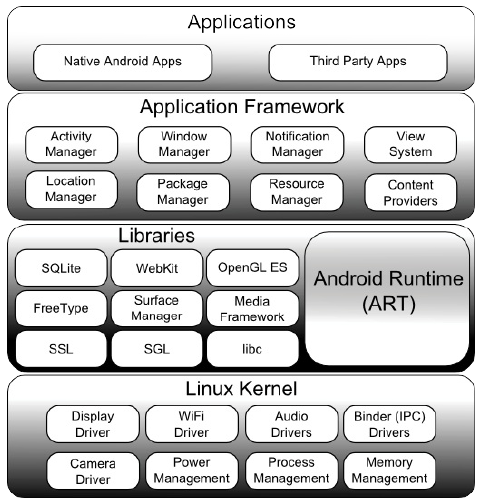
\includegraphics[width=\linewidth]{android_knowledge/os/images/stack.png}
  \caption{Software stack}
  \label{fig:android:sotfware-stack}
\end{figure}


\section{Linux kernel}
 Android uses only the Linux kernel. You can view the Android OS as having two
 distinct sides to it:
\begin{itemize}
    \item a stripped-down and modified Linux kernel 
    \item an application virtual machine that runs Java-like applications.
\end{itemize}

In contrast to conventional Linux computing, each application that is installed
on an Android device is assigned its own unique user identifier (UID) and group
identifier (GID). In certain instances this statement does not hold true and
applications can run under the same user, but these are covered later in this
chapter under the “Application Sandbox” section.

Every Android application has to be given a unique package name by its
developer. The naming convention for these packages should be all lowercase and
the reverse Internet domain name of the organization that developed it
(\verb+com.amazingutils.batterysaver+)

Installed application are assigned a private data directory at the
following location on the  filesystem. 
\begin{verbatim}
shell@android:/ # ls -l /data/data/
...
drwxr-x--x u0_a46 u0_a46 2014-04-10 10:41 com.amazingutils.batterysaver
\end{verbatim}

Notice that the owner of the folder is the newly created user for that
application (\verb+u0_a46+, which translates to \verb+UID 10046+).


\section{Dalvik Virtual Machine (DVM)}
The Dalvik Virtual Machine (DVM) was specifically designed for the Android
platform and is unique to it. The main reason for its existence is that it was
designed to run on hardware with processing and memory constraints and is much
lighter than the normal Java Virtual Machine. It was designed in a way that
allows many Dalvik VMs to be run at the same time in a memory-efficient manner.
The code that runs on it is written and compiled to Java classes and then
converted into a single \verb+DEX+ file using the dx SDK utility. 


\section{Android Runtime (ART)}
When an Android app is built within Android Studio it is compiled into an
intermediate bytecode format (referred to as DEX format). When the
application is subsequently loaded onto the device, the Android Runtime
(ART) uses a process referred to as Ahead-of-Time (AOT) compilation to
translate the bytecode down to the native instructions required by the device
processor. This format is known as Executable and Linkable Format (ELF).

Each time the application is subsequently launched, the ELF executable
version is run, resulting in faster application performance and improved
battery life.

This contrasts with the Just-in-Time (JIT) compilation approach used in
older Android implementations whereby the bytecode was translated within a
virtual machine (VM) each time the application was launched.

\section{Android Libraries}
In addition to a set of standard Java development libraries the Android
development environment also includes the Android Libraries.  A summary of some
key core Android libraries available to the Android developer is as follows:
\begin{itemize}
    \item android.app – Provides access to the application model and is the
        cornerstone of all Android applications.
    \item android.content – Facilitates content access, publishing and
        messaging between applications and application components.a
    \item android.database – Used to access data published by content providers
        and includes SQLite database management classes.
    \item android.graphics – A low-level 2D graphics drawing API including
        colors, points, filters, rectangles and canvases.
    \item android.hardware – Presents an API providing access to hardware such
        as the accelerometer and light sensor.
    \item android.opengl – A Java interface to the OpenGL ES 3D graphics rendering API.
    \item android.os – Provides applications with access to standard operating system services including messages, system services and inter-process communication.
    \item android.media – Provides classes to enable playback of audio and video.
    \item android.net – A set of APIs providing access to the network stack.  Includes android.net.wifi, which provides access to the device’s wireless stack.
    \item android.print – Includes a set of classes that enable content to be sent to configured printers from within Android applications.
    \item android.provider – A set of convenience classes that provide access to standard Android content provider databases such as those maintained by the calendar and contact applications.
    \item android.text – Used to render and manipulate text on a device display.
    \item android.util – A set of utility classes for performing tasks such as string and number conversion, XML handling and date and time manipulation.
    \item android.view – The fundamental building blocks of application user interfaces.
    \item android.widget - A rich collection of pre-built user interface components such as buttons, labels, list views, layout managers, radio buttons etc.
    \item android.webkit – A set of classes intended to allow web-browsing capabilities to be built into applications.
\end{itemize}

It is important to note, however, that the core libraries do not
perform much of the actual work and are, in fact, essentially Java “wrappers”
around a set of C/C++ based libraries.

C/C++ libraries are included to fulfill a wide and diverse range of functions
including 2D and 3D graphics drawing, Secure Sockets Layer (SSL)
communication, SQLite database management, audio and video playback,
bitmap and vector font rendering, display subsystem and graphic layer
management and an implementation of the standard C system library (libc).


In practice, the typical Android application developer will access these
libraries solely through the Java based Android core library APIs. In the event
that direct access to these libraries is needed, this can be achieved using the
Android Native Development Kit (NDK), the purpose of which is to call the
native methods of non-Java or Kotlin programming languages (such as C and
C++) from within Java code using the Java Native Interface (JNI).

\section{Application Framework}
The Application Framework is a set of services that collectively form the
environment in which Android applications run and are managed. This framework
implements the concept that Android applications are constructed from reusable,
interchangeable and replaceable components.  This concept is taken a step
further in that an application is also able to publish its capabilities along
with any corresponding data so that they can be found and reused by other
applications.

The Android framework includes the following key services:

\begin{itemize}
        \item Activity Manager – Controls all aspects of the application
            lifecycle and activity stack.
        \item Content Providers – Allows applications to publish and share data
            with other applications.
        \item Resource Manager – Provides access to non-code embedded resources
            such as strings, color settings and user interface layouts.
        \item Notifications Manager – Allows applications to display alerts and
            notifications to the user.
        \item View System – An extensible set of views used to create
            application user interfaces.
        \item Package Manager – The system by which applications are able to
            find out information about other applications currently installed
            on the device.
        \item Telephony Manager – Provides information to the application about
            the telephony services available on the device such as status and
            subscriber information.
        \item Location Manager – Provides access to the location services
            allowing an application to receive updates about location changes.
\end{itemize}

\section{Applications}
These comprise both the native applications provided with the particular Android
implementation (for example web browser and email applications) and the
third party applications installed by the user after purchasing the device.


\section{Android Applications and Resource Management}

Each running Android application is viewed by the operating system as a
separate process. If the system identifies that resources on the device are
reaching capacity it will take steps to terminate processes to free up memory.

When making a determination as to which process to terminate in order to
free up memory, the system takes into consideration both the priority and
state of all currently running processes, combining these factors to create
what is referred to by Google as an importance hierarchy. Processes are then
terminated starting with the lowest priority and working up the hierarchy 
until sufficient resources have been liberated for the system to function.

\subsection{Android Process States}
Processes host applications and applications are made up of components.
Within an Android system, the current state of a process is defined by the
highest-ranking active component within the application that it hosts. A
process can be in one of the following five states at any given time ordered by
higher to lower priority
\subsubsection{Foreground Process}
These processes are assigned the highest level of priority. At any one time,
there are unlikely to be more than one or two foreground processes active and
these are usually the last to be terminated by the system. A process must meet
one or more of the following criteria to qualify for foreground status:
\begin{itemize}
        \item Hosts an activity with which the user is currently interacting.
        \item Hosts a Service connected to the activity with which the user is interacting.
        \item Hosts a Service that has indicated, via a call to
            \verb+startForeground()+, that termination would be disruptive to the user experience.
        \item Hosts a Service executing either its \verb+onCreate()+,
            \verb+onResume()+ or \verb+onStart()+ callbacks.
        \item Hosts a Broadcast Receiver that is currently executing its
            \verb+onReceive()+ method.
\end{itemize}

\subsubsection{Visible Process}
A process containing an activity that is visible to the user but is not the
activity with which the user is interacting is classified as a “visible process”.
This is typically the case when an activity in the process is visible to the user
but another activity, such as a partial screen or dialog, is in the foreground. A
process is also eligible for visible status if it hosts a Service that is, itself, bound
to a visible or foreground activity.

\subsubsection{Service Process}

Processes that contain a Service that has already been started and is currently
executing.

\subsubsection{Background Process}
A process that contains one or more activities that are not currently visible to
the user, and does not host a Service that qualifies for Service Process status.
Processes that fall into this category are at high risk of termination in the
event that additional memory needs to be freed for higher priority processes.
Android maintains a dynamic list of background processes, terminating
processes in chronological order such that processes that were the least
recently in the foreground are killed first.

\subsubsection{Empty Process}

Empty processes no longer contain any active applications and are held in
memory ready to serve as hosts for newly launched applications. This is
somewhat analogous to keeping the doors open and the engine running on a
bus in anticipation of passengers arriving. Such processes are, obviously,
considered the lowest priority and are the first to be killed to free up
resources.

\subsection{Inter-Process Dependencies}

The situation with regard to determining the highest priority process is
slightly more complex than outlined in the preceding section for the simple
reason that processes can often be inter-dependent. As such, when making a
determination as to the priority of a process, the Android system will also
take into consideration whether the process is in some way serving another
process of higher priority (for example, a service process acting as the content
provider for a foreground process). As a basic rule, the Android
documentation states that a process can never be ranked lower than another
process that it is currently serving.


